\section{Model of use}

The proposed offload mechanism implements the OpenMP 4.0 \dtargetdata{}, \dtarget{} and \ddeclaretarget{} constructs. The compiler generates calls to the runtime library whenever a \dtargetdata{} or \dtarget{} directive is encountered. The \ddeclaretarget{} construct will result in the generation of appropriate target code for the target device.

The target code is stored inside the host binaries as additional ELF sections with an appropriate naming convention. The target code is either target assembly in binary form (ELF, PE, etc.) or a higher-level intermediate representation (IR) such as LLVM IR or any other type of IR. If the target code is stored as IR, an implementation can support on-the-fly compilation into target assembly. Note that ELF terminology is being used throughout the document only for illustrative purposes $-$ the implementation should accommodate any other object format supported by LLVM.

A target-independent offload runtime library named \libomptarget{} supports multiple target device types. The \libomptarget{} library utilizes device-specific target run-time libraries (RTLs). At the start of host code execution \libomptarget{} will do the following:

\begin{enumerate}
  \item Search for target RTLs according to a naming convention. 

  \item Verify target RTL interface compliance.

  \item Add target RTLs into a list of available target device types. 
\end{enumerate}

The \libomptarget{} provides the host with an API to map variables and initiate execution of target regions on a target device. After the \libomptarget{} has verified that suitable target code is present and that a target RTL is ready to execute a target region, the target RTL is invoked via API routines(described below) to execute the region.

This scheme provides flexibility for generating code for multiple heterogeneous device types. For example, the target region code in Example~\ref{ex:OffloadingExample} can be executed in a Phi\texttrademark{} coprocessor if it is present on user’s system or on a GPU system if it is present (see Figure~\ref{fg:libomptarget_schematic}). The design of the offloading interface does not limit the number and type of devices associated to a host processor or the ability to use these at the same time. If both devices are present, different iterations of the loop can be executed on both devices at the same time.

\begin{figure}
  \centering
  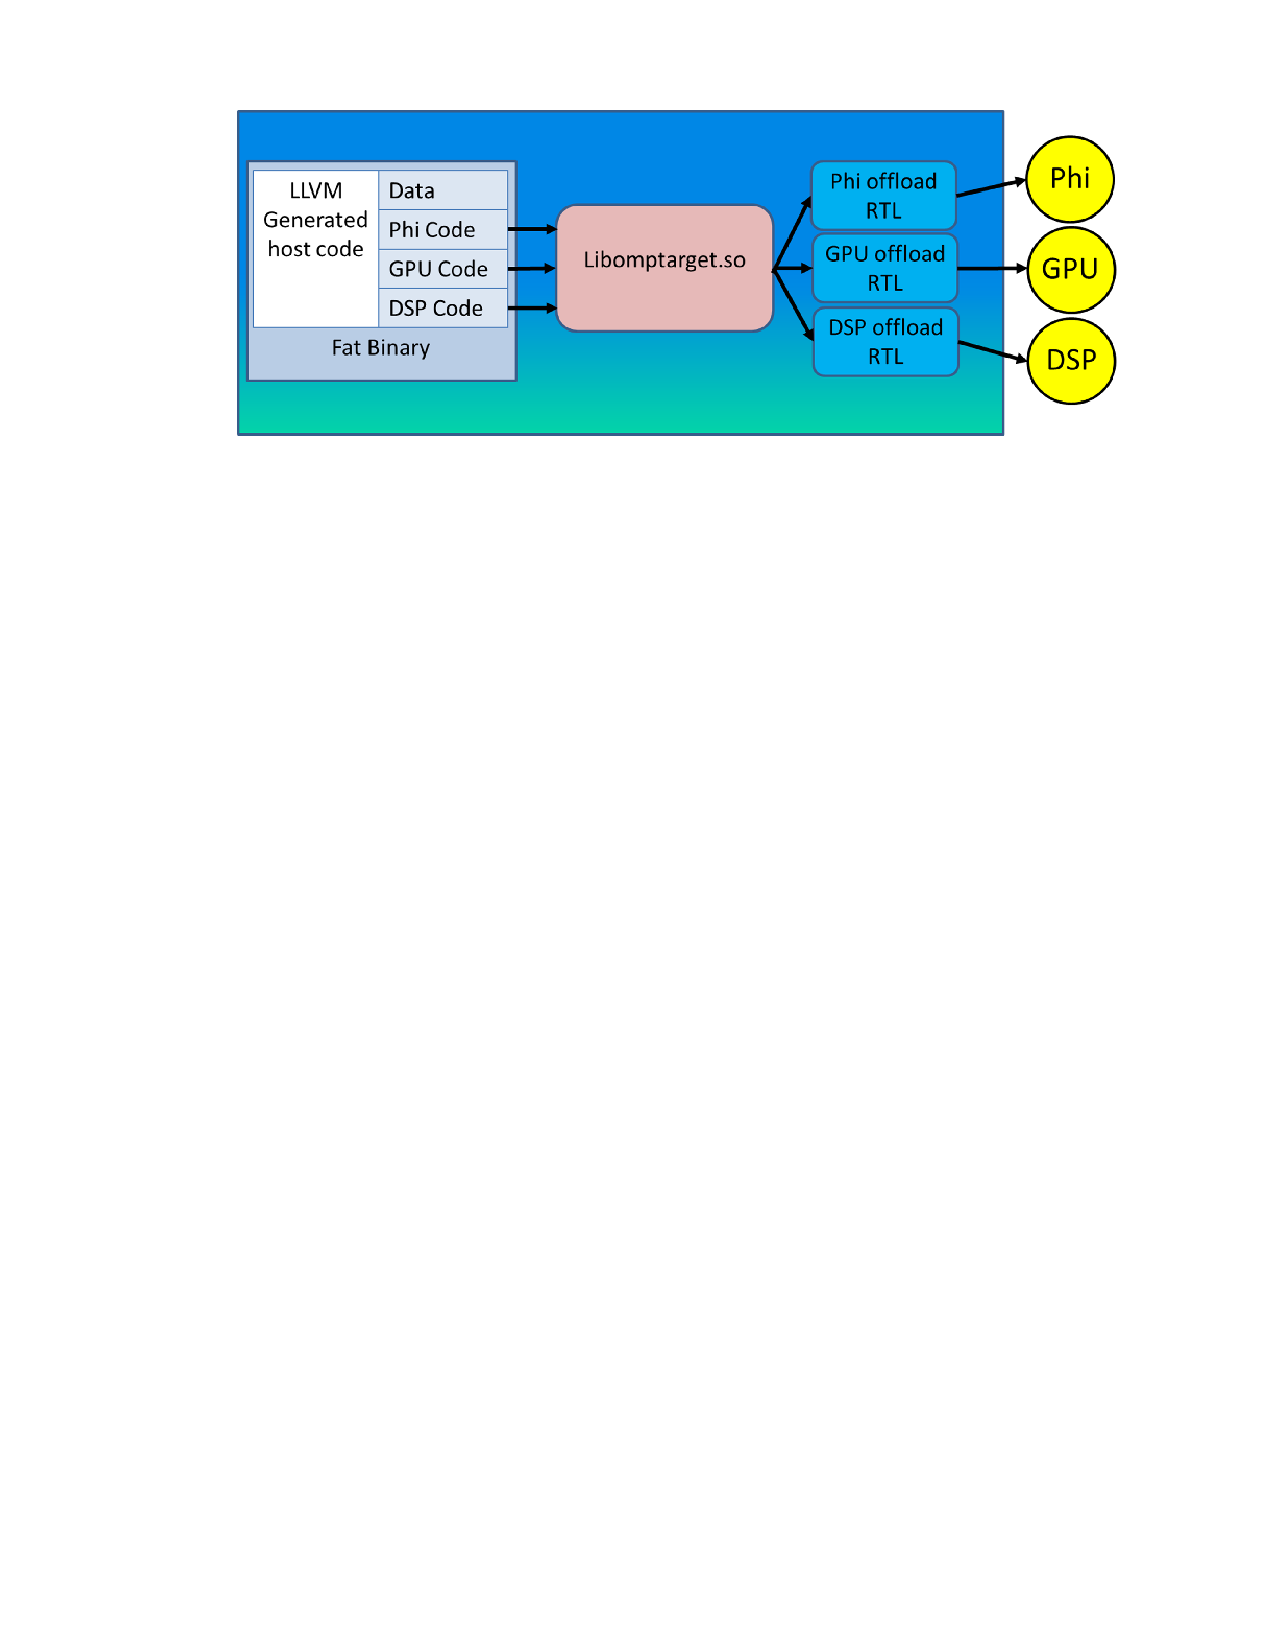
\includegraphics[width=0.9\textwidth]{ImageLibomptarget.pdf}
  \caption{Schematic of libomptarget.so interface}
  \label{fg:libomptarget_schematic}
\end{figure}
